\documentclass[tikz,border=10pt]{standalone}
\usepackage{tikz}
\usetikzlibrary{shadows,shapes,arrows,positioning,fit,backgrounds,decorations.pathreplacing,calc}

% Define colors
\definecolor{tsgblue}{RGB}{66, 133, 244}     % Core Format
\definecolor{tsggreen}{RGB}{52, 168, 83}     % Core Tool
\definecolor{tsgyellow}{RGB}{251, 188, 5}    % API/Bindings
\definecolor{tsgpurple}{RGB}{103, 58, 183}   % Applications
\definecolor{tsgred}{RGB}{234, 67, 53}       % Language Bindings
\definecolor{tsgcyan}{RGB}{0, 151, 167}      % Format Conversion
\definecolor{tsgindigo}{RGB}{63, 81, 181}    % Format Types
\definecolor{tsgorange}{RGB}{255, 87, 34}    % End Users
\definecolor{tsggray}{RGB}{102, 102, 102}    % Connectors

\begin{document}

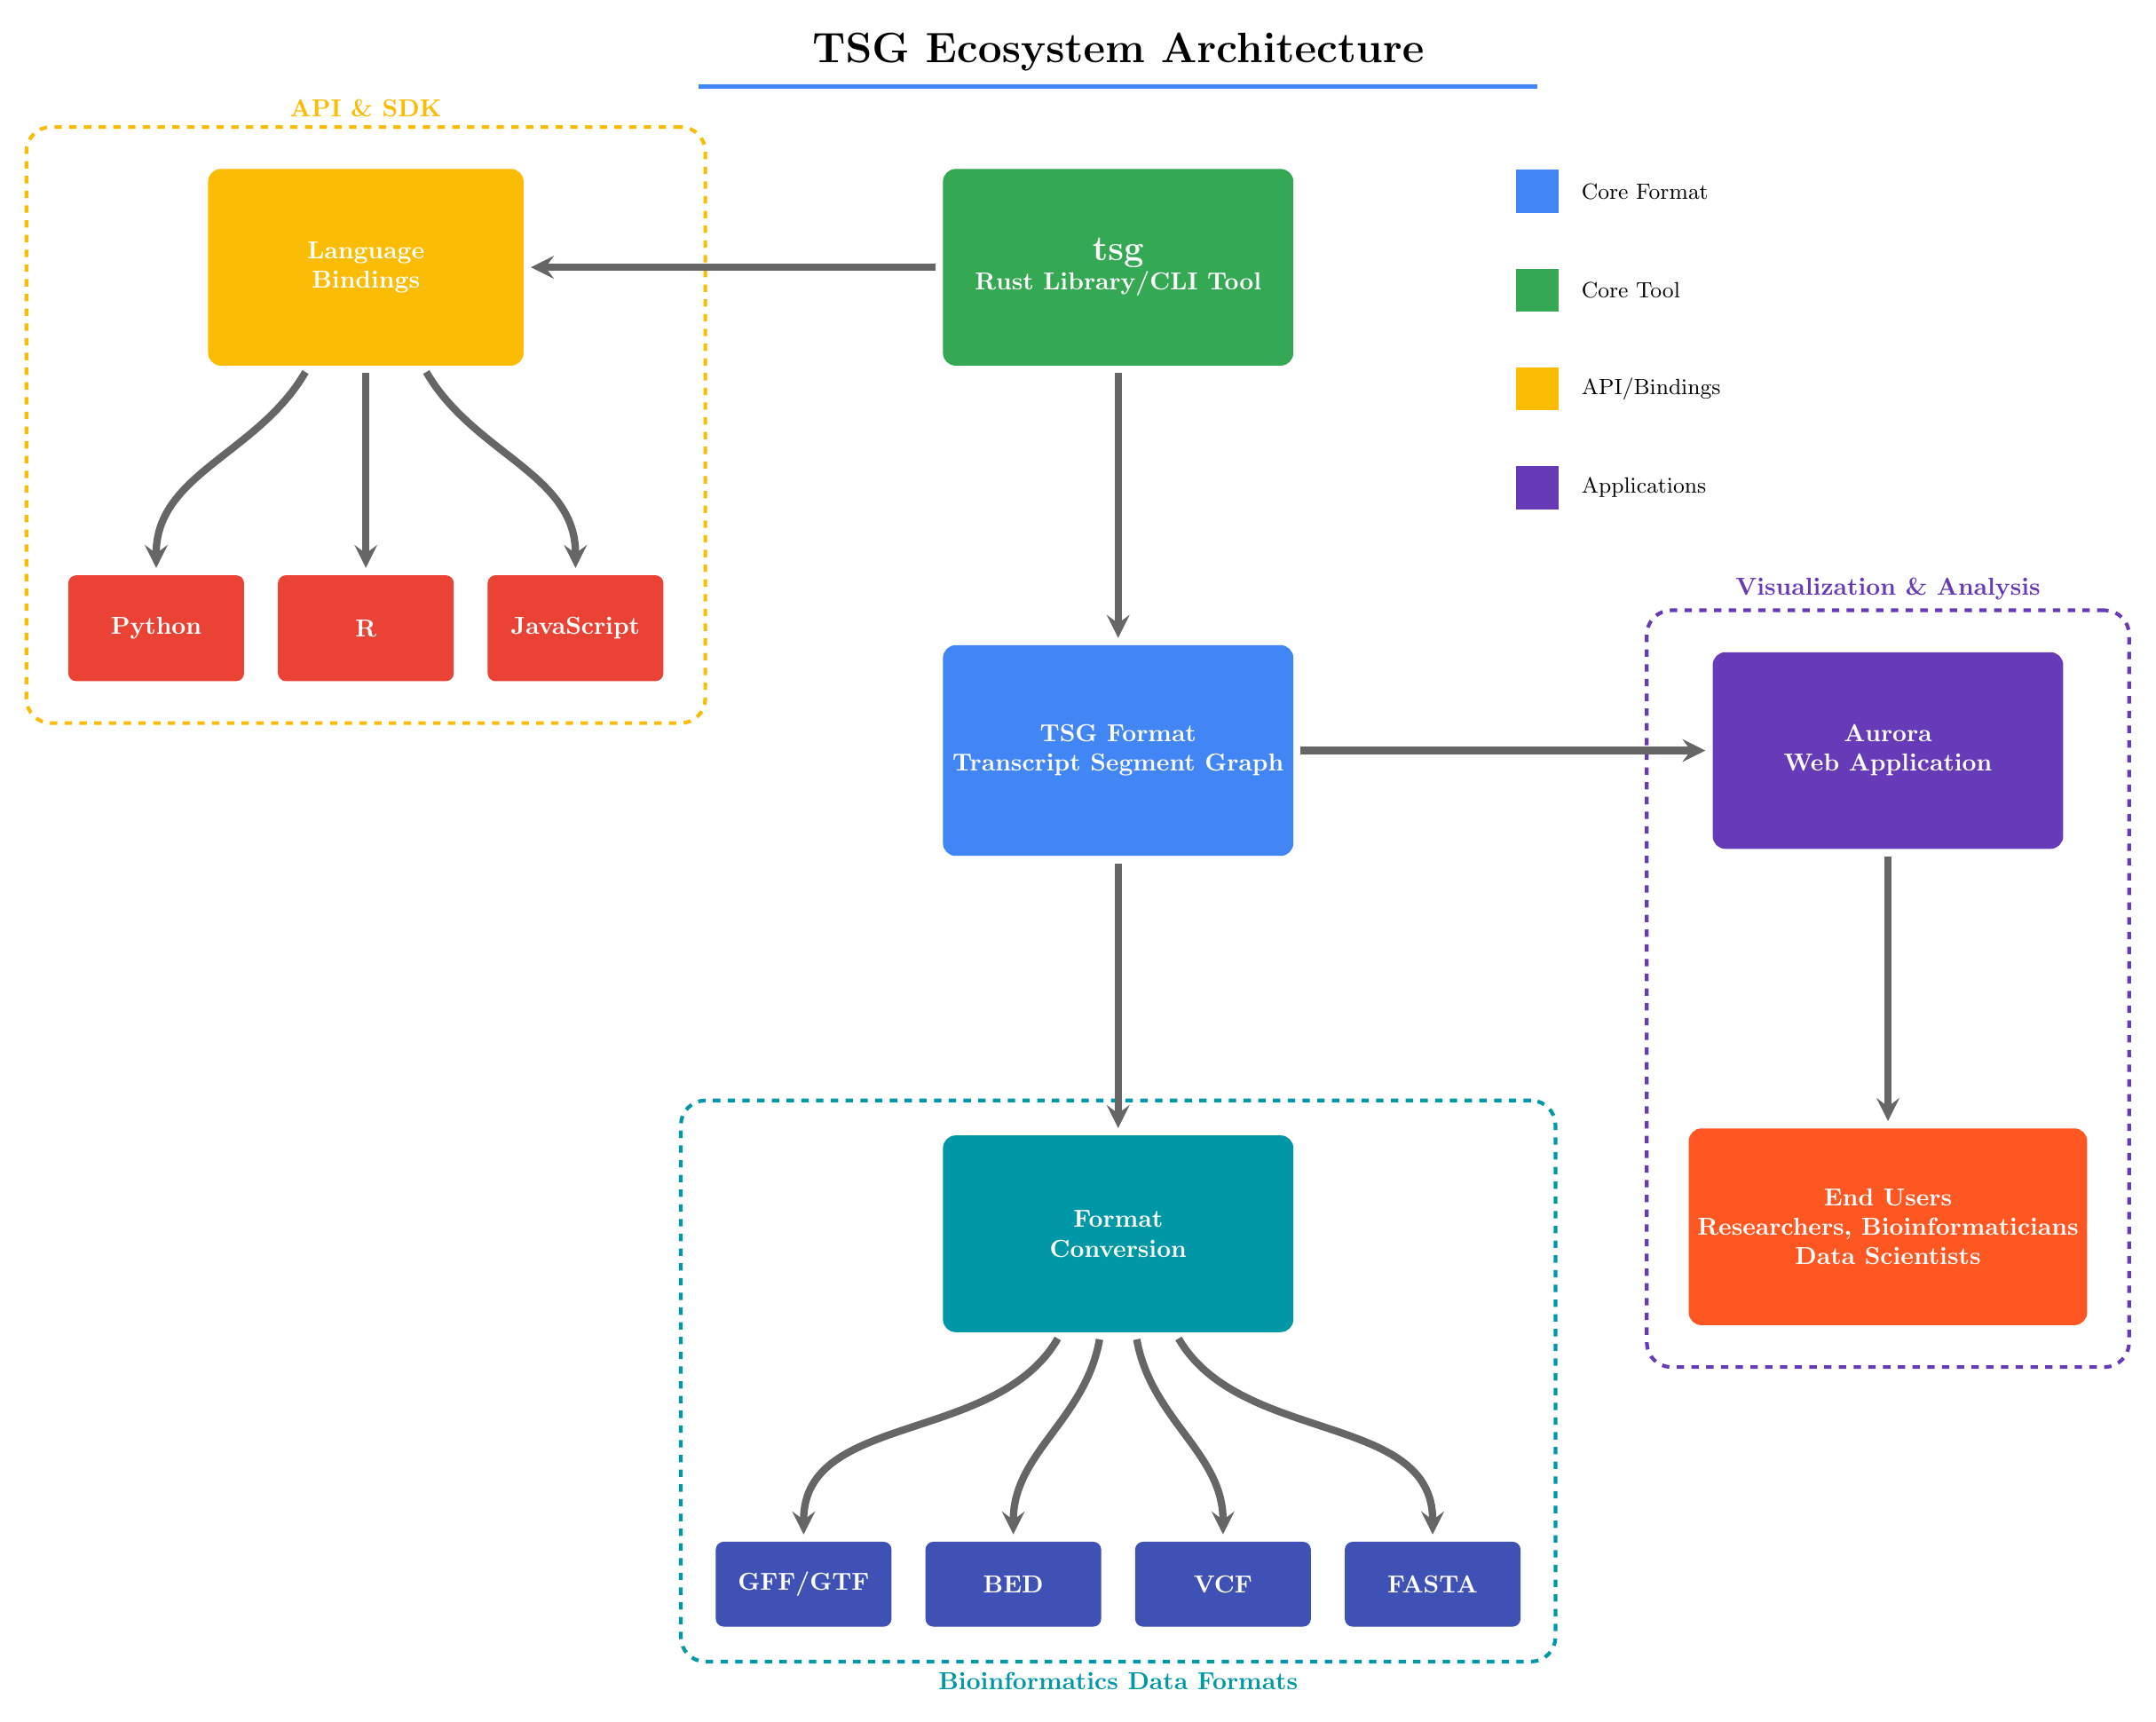
\begin{tikzpicture}[
		% Node styles
		format/.style={draw=tsgblue, fill=tsgblue, text=white, rounded corners=5pt,
				minimum width=5cm, minimum height=3cm, font=\bfseries,  align=center},
		tool/.style={draw=tsggreen, fill=tsggreen, text=white, rounded corners=5pt,
				minimum width=5cm, minimum height=2.8cm, font=\bfseries, align=center},
		binding/.style={draw=tsgyellow, fill=tsgyellow, text=white, rounded corners=5pt,
				minimum width=4.5cm, minimum height=2.8cm, font=\bfseries, align=center},
		app/.style={draw=tsgpurple, fill=tsgpurple, text=white, rounded corners=5pt,
				minimum width=5cm, minimum height=2.8cm, font=\bfseries, align=center},
		lang/.style={draw=tsgred, fill=tsgred, text=white, rounded corners=3pt,
				minimum width=2.5cm, minimum height=1.5cm, font=\bfseries, align=center},
		conversion/.style={draw=tsgcyan, fill=tsgcyan, text=white, rounded corners=5pt,
				minimum width=5cm, minimum height=2.8cm, font=\bfseries,  align=center},
		format_type/.style={draw=tsgindigo, fill=tsgindigo, text=white, rounded corners=3pt,
				minimum width=2.5cm, minimum height=1.2cm, font=\bfseries, align=center},
		user/.style={draw=tsgorange, fill=tsgorange, text=white, rounded corners=5pt,
				minimum width=5cm, minimum height=2.8cm, font=\bfseries,  align=center},
		connector/.style={->, >=stealth, draw=tsggray, line width=3pt, shorten >=3pt, shorten <=3pt},
		groupbox/.style={draw=#1, dashed, rounded corners=10pt, line width=1pt},
		title/.style={font=\LARGE\bfseries},
		subtitle/.style={font=\small},
		legend_box/.style={draw=#1, fill=#1, minimum width=0.6cm, minimum height=0.6cm},
		% Define node distances
	]

	\pgfdeclarelayer{background}
	\pgfsetlayers{background,main}

	% Title - positioned at the top center
	\node[title] (title) at (0,10) {TSG Ecosystem Architecture};
	\draw[tsgblue, line width=1.5pt] (-6,9.5) -- (6,9.5);

	% Start with the core format as the center reference point
	\node[format] (tsg_format) at (0,0) {TSG Format \\ Transcript Segment Graph};

	% Position other main components relative to core format
	\node[tool] (tsg_tool) [above=4cm of tsg_format] {\Large tsg \\ Rust Library/CLI Tool};
	\node[binding] (bindings) [left=6cm of tsg_tool] {Language \\ Bindings};
	\node[app] (aurora) [right=6cm of tsg_format] {Aurora \\ Web Application};
	\node[conversion] (conversion) [below=4cm of tsg_format] {Format \\ Conversion};
	\node[user] (users) [below=4cm of aurora] {End Users \\ Researchers, Bioinformaticians \\ Data Scientists};

	% Language bindings positioned relative to bindings node - aligned horizontally
	\node[lang] (python) [below=3cm of bindings, xshift=-3cm] {Python};
	\node[lang] (r) [below=3cm of bindings] {R};
	\node[lang] (js) [below=3cm of bindings, xshift=3cm] {JavaScript};

	% Format types positioned relative to conversion node
	\node[format_type] (gff) [below=3cm of conversion, xshift=-4.5cm] {GFF/GTF};
	\node[format_type] (bed) [below=3cm of conversion, xshift=-1.5cm] {BED};
	\node[format_type] (vcf) [below=3cm of conversion, xshift=1.5cm] {VCF};
	\node[format_type] (fasta) [below=3cm of conversion, xshift=4.5cm] {FASTA};


	% Connections
	\draw[connector] (tsg_tool) -- (tsg_format);
	\draw[connector] (tsg_tool) -- (bindings);
	\draw[connector] (tsg_format) -- (aurora);
	\draw[connector] (tsg_format) -- (conversion);
	\draw[connector] (aurora) -- (users);

	% Bindings to languages
	\draw[connector] (bindings) to[out=-120, in=90] (python);
	\draw[connector] (bindings) to[out=-90, in=90] (r);
	\draw[connector] (bindings) to[out=-60, in=90] (js);

	% Format Conversion to formats
	\draw[connector] (conversion) to[out=-120, in=90] (gff);
	\draw[connector] (conversion) to[out=-100, in=90] (bed);
	\draw[connector] (conversion) to[out=-80, in=90] (vcf);
	\draw[connector] (conversion) to[out=-60, in=90] (fasta);

	% Group boxes in background
	\begin{pgfonlayer}{background}
		\node[fit=(bindings) (python) (r) (js), groupbox=tsgyellow, inner sep=0.6cm, line width=1.5pt,
			label={[tsgyellow, font=\bfseries]above:API \& SDK}] {};
		\node[fit=(aurora) (users), groupbox=tsgpurple, inner sep=0.6cm, line width=1.5pt,
			label={[tsgpurple, font=\bfseries]above:Visualization \& Analysis}] {};
		\node[fit=(conversion) (gff) (bed) (vcf) (fasta), groupbox=tsgcyan, inner sep=0.5cm, line width=1.5pt,
			label={[tsgcyan, font=\bfseries]below:Bioinformatics Data Formats}] {};
	\end{pgfonlayer}

	% Legend - positioned relative to top right
	\node[legend_box=tsgblue] (legend1) at (6,8) {};
	\node[right=0.2cm of legend1, font=\small] {Core Format};

	\node[legend_box=tsggreen] (legend2) [below=0.8cm of legend1] {};
	\node[right=0.2cm of legend2, font=\small] {Core Tool};

	\node[legend_box=tsgyellow] (legend3) [below=0.8cm of legend2] {};
	\node[right=0.2cm of legend3, font=\small] {API/Bindings};

	\node[legend_box=tsgpurple] (legend4) [below=0.8cm of legend3] {};
	\node[right=0.2cm of legend4, font=\small] {Applications};

\end{tikzpicture}

\end{document}